
\chapter{Similarity Analysis}\label{simanal}

%\textit{\textbf{This needs an introduction, the smaller the distance the more similar the songs are etc. -> smilarity = 1 / distance}}

\section{Timbre Similarity} \label{musly}

This section focuses on different similarity measurements and metrics based on MFCCs. Mel Frequency Cepstral Coefficients have already been introduced in Section \ref{mfccsim} as a feature to describe timbre.\\

\subsection{Euclidean Distance}\label{mfcceuc}

To further reduce the dimensionality of the original MFCC features, a statistical summarization can be calculated. For each of the Mel-bands (13 in this case) the mean and standard deviation over all frames is calculated, resulting in a vector of 13 mean values, a 13 by 13 covariance matrix ($\frac{13*(13-1)}{2}$ covariance values, because of the triangular shape - the upper triangle contains the covariances and the main diagonal contains the variances) and 13 variances. These vectors are not dependent on the length of the actual song. \cite[pp. 51ff]{knees1}\\
Using such a model, the distance between two songs can be calculated using the $L_p$ distance as in equation \ref{eq:distGmm}, where x and y are the n-dimensional feature vectors of two different musical pieces:
\begin{equation} \label{eq:distGmm}
%p (v \vert \lambda)=\sum_{i=1}^{M}w_iN(v \vert \mu_i,\sum_i) \label{prob}
d(x, y) = ||x - y||_p = \left(\sum_{i=1}^{n}{|x_i - y_i|^p}\right)^{\frac{1}{p}}
\end{equation}
Most of the times, the Euclidean ($L_2$) or the Manhattan ($L_1$) distance would be used in real-world scenarios. \cite[p. 58]{knees1}\\
This very basic metric of timbre similarity has been refined and improved over the past years.

\subsection{Single Gaussian Model}

\subsubsection{Symmetric Kullback-Leibler Divergence}\label{klth}

The second approach was first proposed by Mandel and Ellis in 2005 \cite{mandelellis1} and is briefly summarized in \cite[pp. 65f]{knees1}.\\
After computing the mean value of each MFCC ($\mu_P$ and $\mu_Q$) and the covariance matrix of the different MFCC vectors ($\Sigma_P$ and $\Sigma_Q$) of two musical pieces $P$ and $Q$, the Kullback-Leibler divergence (KL divergence) can be calculated as follows, with $tr(\cdot)$ being the trace (i.e., the sum of the diagonal of a matrix), $d$ being the dimensionality (number of MFCCs) and $|\Sigma_P|$ being the determinant of $\Sigma_P$.\\
\begin{equation} \label{eq:KL1}
KL_{(P||Q)} = \frac{1}{2}[log\frac{|\Sigma_P|}{|\Sigma_Q|} + tr(\Sigma_P^{-1}\Sigma_Q) + (\mu_P - \mu_Q)^T \Sigma_P^{-1} (\mu_Q - \mu_P) - d]
\end{equation}
As a second step the result has to be symmetrized.
\begin{equation} \label{eq:KL2}
d_{KL}(P, Q) = \frac{1}{2} (KL_{(P||Q)} + KL_{(Q||P)}) 
\end{equation}
This approach is one of the two available similarity metrics in the Musly \cite{musly1} toolkit (see Section \ref{mirtoolkit}). It can be simplified and written as a closed form according to \cite[p. 44]{schnitzer1}:
\begin{equation} \label{eq:SKL}
d_{SKL}(P, Q) = \frac{1}{4} (tr(\Sigma_P\Sigma_Q^{-1}) + tr(\Sigma_Q\Sigma_P^{-1}) + tr((\Sigma_Q^{-1}\Sigma_P^{-1})(\mu_P - \mu2)^2) - 2d)
\end{equation}

\subsubsection{Jensen-Shannon-Like Divergence}

The second available similarity method in the Musly toolkit by Schnitzer is using the Jensen-Shannon divergence (in a slightly adapted way). "The Jensen-Shannon (JS) divergence is another symmetric divergence derived from the Kullback-Leibler divergence. To compute it, a mixture $X_m$ of the two distributions is defined" \cite[p. 43]{schnitzer1}. "To use the Jensen-Shannon divergence [...] to estimate similarities between Gaussians, an approximation of $X_m$ as a single multivariate Gaussian can be used [...] This approximation of $X_m$ is exactly the same as the left-type Kullback-Leibler centroid of the two Gaussian distributions [...]" \cite[p. 45]{schnitzer1} 
\begin{equation} \label{eq:jsl1}
\mu_m = \frac{1}{2} \mu_P + \frac{1}{2} \mu_Q
\end{equation}
\begin{equation} \label{eq:jsl2}
\Sigma_m = \frac{1}{2} (\Sigma_P + \mu_P\mu_P^T) + \frac{1}{2} (\Sigma_Q + \mu_Q\mu_Q^T) - \mu_m\mu_m^T
\end{equation}
\begin{equation} \label{eq:jsl3}
JS(P, Q) = \frac{1}{2} log|\Sigma_m| - \frac{1}{4} log |\Sigma_P| - \frac{1}{4} log |\Sigma_Q|
\end{equation}

\subsubsection{Mutual Proximity}\label{mprox}
After calculating a similarity matrix for all songs, Musly normalizes the similarities with mutual proximity (MP). \cite{musly2}. This method wants to reduce the effect of a phenomenon called "hubness", which appears as a general problem of machine learning in high-dimensional data spaces. "Hubs are data points which keep appearing unwontedly often as nearest neighbors of a large number of other data points." \cite[p. 66]{schnitzer1}.\\
Schedl and Knees state: "To apply MP to a distance matrix, it is assumed that the distances $D_{x,i = 1..N}$ from an object $x$ to all other objects in the data set follow a certain probability distribution; thus, any distance $D_{x,y}$ can be reinterpreted as the probability of $y$ being the nearest neighbor of $x$, given the distance $D_{x,y}$ and the probability distribution $P(x)$ [...] MP is then defined as the probability that $y$ is the nearest neighbor of $x$ given $P(x)$ and $x$ is the nearest neighbor of $y$ given $P(y)$" \cite[p. 80]{knees1}\\
Resulting in: 
\begin{equation} \label{eq:mp1}
P(X > D_{x,y}) = 1 - P(X \leq D_{x,y}) = 1 - \mathscr{F}(D_{x,y}) 
\end{equation}
\begin{equation} \label{eq:mp2}
MP(D_{x,y}) = P(X > D_{x,y} \cap Y > D_{x,y})
\end{equation}
according to \cite[p. 80]{knees1}\\
%Because in this thesis the full similarity matrix is not calculated, 

\subsection{Gaussian Mixture Models and Block-Level Features}\label{blocklevel}
Another, more compute-heavy distance measurement would make use of Gaussian Mixture Models (GMMs) of MFCCs. As Knees and Schedl state "Other work on music audio feature modeling for similarity has shown that aggregating the MFCC vectors of each song via a single Gaussian may work almost as well as using a GMM [...] Doing so decreases computational complexity by several magnitudes, in comparison to GMM-based similarity computations." \cite[p. 65]{knees1} Therefore, the usage of GMMs is not further considered in this thesis.\\
The last method mentioned, but not implemented in this thesis for timbral similarity uses block-level features as proposed by Seyerlehner \cite{seyerlehnerblock} and described in short by Knees and Schedl \cite[p. 67]{knees1}. Instead of using single frames and summarizing them into statistical or probabilistic models, block-level features use larger, e.g., multiple-second long, audio frames. Features like fluctuation patterns (later introduced in Section \ref{flucpat}) and spectral patterns (containing timbre information) are computed for these larger blocks of frames. 

\subsection{Validation}

For this thesis, the Kullback-Leibler divergence, the Jensen-Shannon divergence and the Euclidean distance are chosen and tested. There is always a trade-off between the complexity and functionality of the distance computing algorithms and a re-implementation of the block-level features remains left open for future research due to its rather compute heavy nature.\\
Using the Musly toolkit, a first evaluation unsing the symmetric KL divergence is presented in this section. The feature extraction and distance calculation can also be done in python using the librosa library, and a small re-implementation of the Mandel-Ellis approach was tested as well.\\

\subsubsection{Genre Recall Rate/ Construction Noise}
In general, a good measurement for the efficiency of timbre similarity algorithms, is the ability to recommend songs of the same genre. 
Alternatively, the example proposed by Dr. Bosse from the introduction was tested (see Chapter \ref{intro}). Comparing a construction noise sound sample with the private music collection containing mostly metal, rock, pop, classical and hip hop music, the following six best results were returned in descending order: 

\begin{itemize}
	\setlength\itemsep{-0.5em}
	\item Ziegenm\"uhlen Session - Down On The Corner (Folk Musik)
	\item While She Sleeps - The Divide (Metalcore)
	\item Delain - Mother Machine (Live) (Symphonic Metal)
	\item Within Temptation - Sanctuary (Intro Live) (Symphonic Metal)
	\item Without A Martyr - Medusa's Gaze (Death Metal)
	\item 100 Meisterwerke der Klassik - Orpheus In The Underworld (Orph\'ee aux enfers) - Can-Can (Live At Grosser Saal, Musikverein) (Klassik)
\end{itemize}

Figure \ref{const1} and \ref{const2} show the distribution of the genres of 100 most similar songs compared to the construction noise sample.  

\begin{figure}[htbp]
	\centering
	\framebox{\parbox{1\textwidth}{ 
			\begin{subfigure}{0.49\textwidth}
				\centering      
				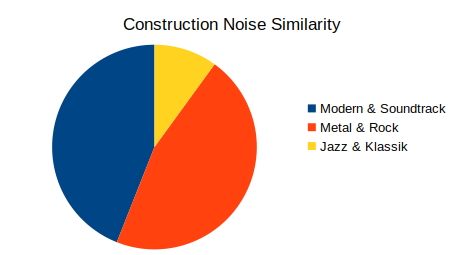
\includegraphics[scale=0.55]{Images/cnoise1.png}
				\caption{Similar genres ()}
				\label{const1}
			\end{subfigure}%
			\begin{subfigure}{0.49\textwidth}
				\centering 
				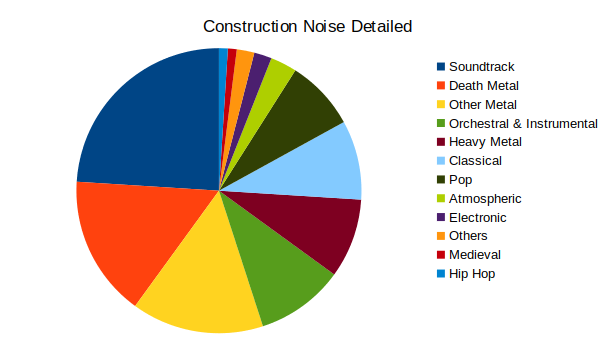
\includegraphics[scale=0.45]{Images/cnoise2.png}
				\caption{Similar genres (detailed)}
				\label{const2}
			\end{subfigure}
	}}
	\caption{Construction Noise}
	\label{fig:constn}
\end{figure}

\noindent Using an extended dataset consisting of the private music collection, private field recordings, the full FMA dataset, and the musicnet data, the following results could be achieved: 

\begin{itemize}
	\setlength\itemsep{-0.5em}
	\item Born Pilot - Birds Fell (FMA, Electronic, Noise)
	\item mrandmrsBrian - sun is boring (FMA, Avant-Garde, field recordings)
	\item steps in snow (private field recording)
	\item Sawako - Paris Children (FMA, field recordings)
	\item Jeremy Gluck and Michael Dent - Olivier (FMA, Ambient Electronic)
\end{itemize}

\noindent Especially the second test shows, that the timbre based recommendations are able to recommend similar sounding audio files by returning mostly music containing ambient noises once these were included to the dataset.

\subsubsection{Different Recordings and Cover Versions}\label{covermfcc}
Another experiment was, to get the most similar songs to the famous 'Rondo alla Turca' by Mozart.
The recording used as a starting point was taken from the CD "100 Meisterwerke der Klassik" and has a length of 3:33 minutes. This piece by Mozart appears overall four times in the dataset and is recorded by different pianists.
Every recording has a different length as listed in the following overview of the recordings by CD.

\begin{itemize}
	\setlength\itemsep{-0.5em}
	\item 100 Meisterwerke der Klassik (3:33)
	\item Piano Perlen (3:30)
	\item The Piano Collection - Disk 18 (3:28)
	\item Mozart Premium Edition - Disk 31 (4:29)
	
\end{itemize}

\noindent The top ten most similar songs to the 3 minutes and 33 seconds version are listed below:

\begin{itemize}
	\setlength\itemsep{-0.5em}
	\item Mozart - Concert No. 10 for 2 Pianos and Orchestra in E Flat Major, KV 365 - 2. Andante
	\item Schubert - Sonata in B Flat, D. 960 - III. Scherzo (Allegro vivace con delicatezza)
	\item Albeniz - Iberia, Book I - Evocaci\'on
	\item \underline{Mozart Sonate Nr. 11 in A-Dur, K. 33 - Mozart - Alla Turca Allegretto (3:28)}
	\item Beethoven - Bagatellen Op 119 -Allemande in D major
	\item Mozart - Rondo No. 1 in D Major, K. 485
	\item Mozart - Sonata For Piano No. 8 KV 310 A Minor - Allegro Maestoso
	\item Sonata For Piano No. 16 KV 545 C Major - Rondo: Allegretto
	\item \underline{Mozart Sonate Nr. 11 in A-Dur, K. 33 - III. Tuerkischer Marsch (3:30)}
	\item Mozart - Piano Sonata No. 13 in B flat major, K. 333 (K. 315c): Allegretto grazioso
	
\end{itemize}
\noindent The interesting conclusion is that only two out of the three other versions were considered as most similar songs. The other recording wasn't even in the top 30 list of the most similar songs. However, the recommendations are all from the same genre (classical music). The inability to detect cover versions was also observable for other songs in the dataset like Serj Tankians song "Lie Lie Lie" from the CD "Harakiri" and an orchestral recording of the same piece. This is probably due to the usage of MFCCs valuing the timbre of the music predominantly instead of the pitches and melody movements. 

